\section{Sequence Diagrams Specification}
\label{appendix:sequence-diagrams}
\subsubsection{Authentication}
This sequence diagram maps the execution flow of the user authentication process.

\begin{figure}[H]
    \centering
    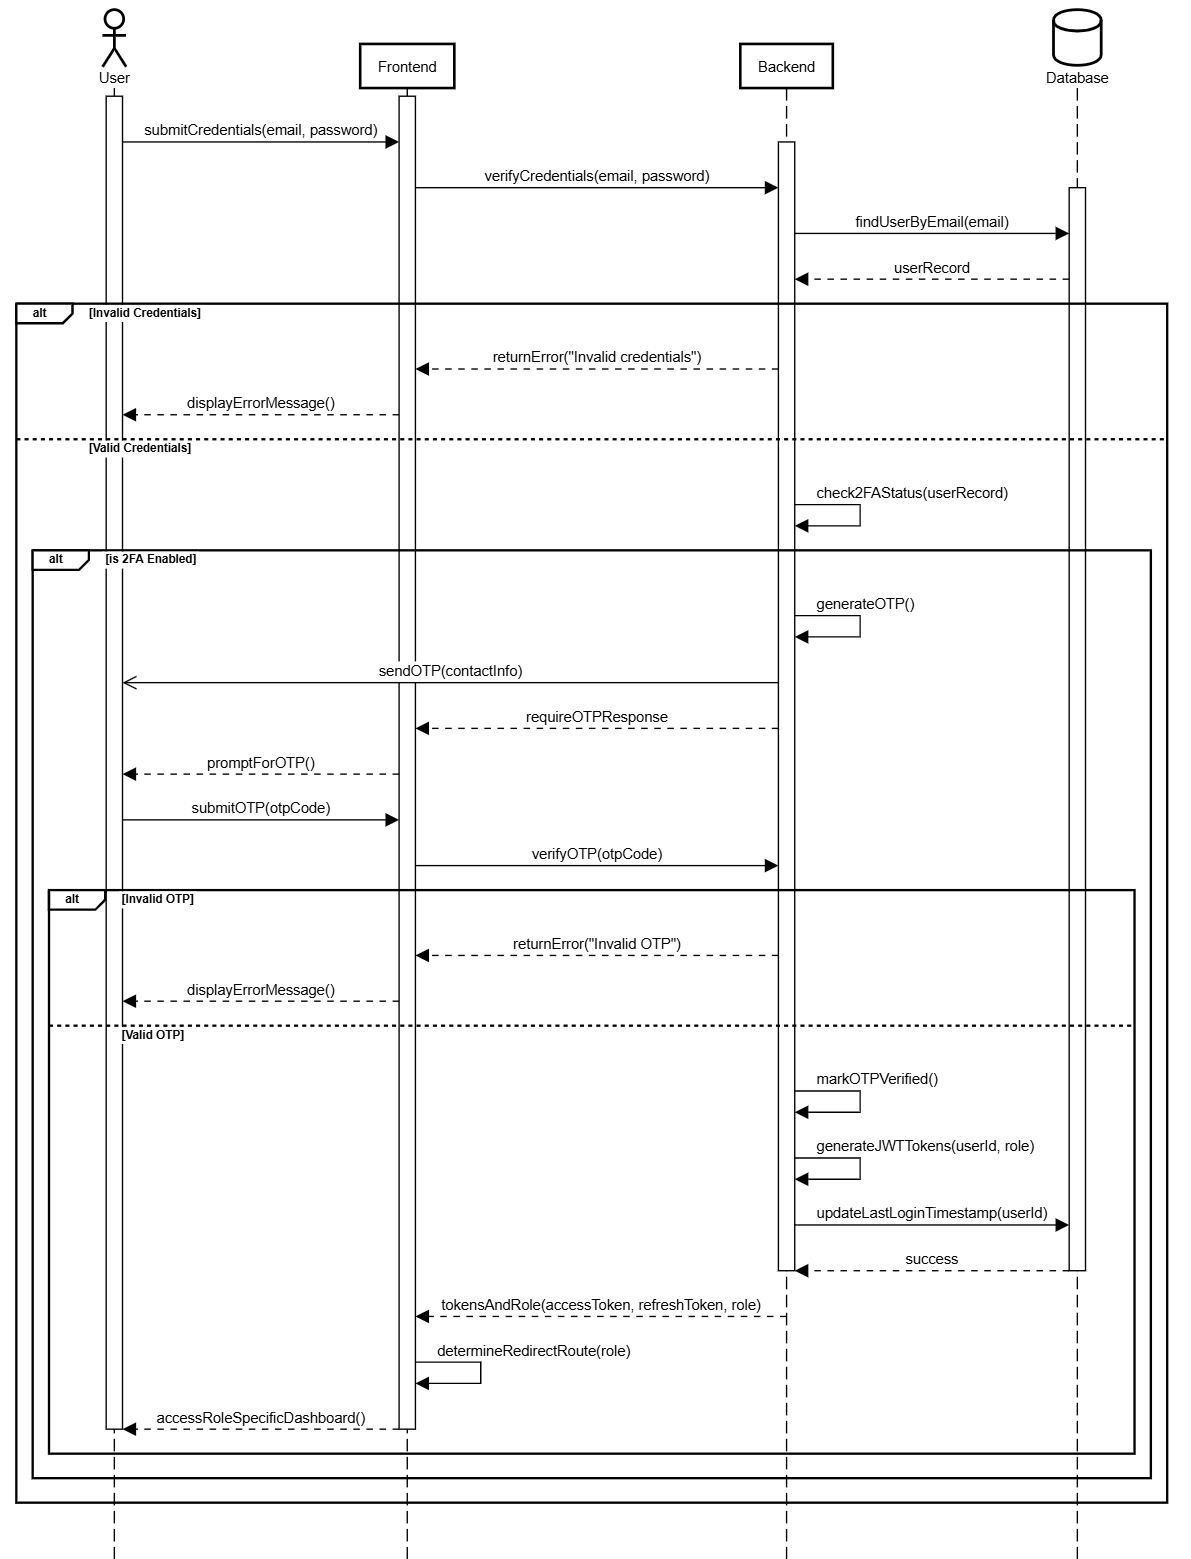
\includegraphics[width=0.95\textwidth]{graphics/seq-diagrams/seq_auth.png}
    \caption{Sequence Diagram: Authentication}
    \label{fig:seq_auth}
\end{figure}


\subsubsection{Smart Content Ingestion}
This sequence details the interactions when a teacher uploads course materials. It highlights the asynchronous chunking, embedding generation, and vector storage processes required to build the RAG pipeline.

\begin{figure}[H]
    \centering
    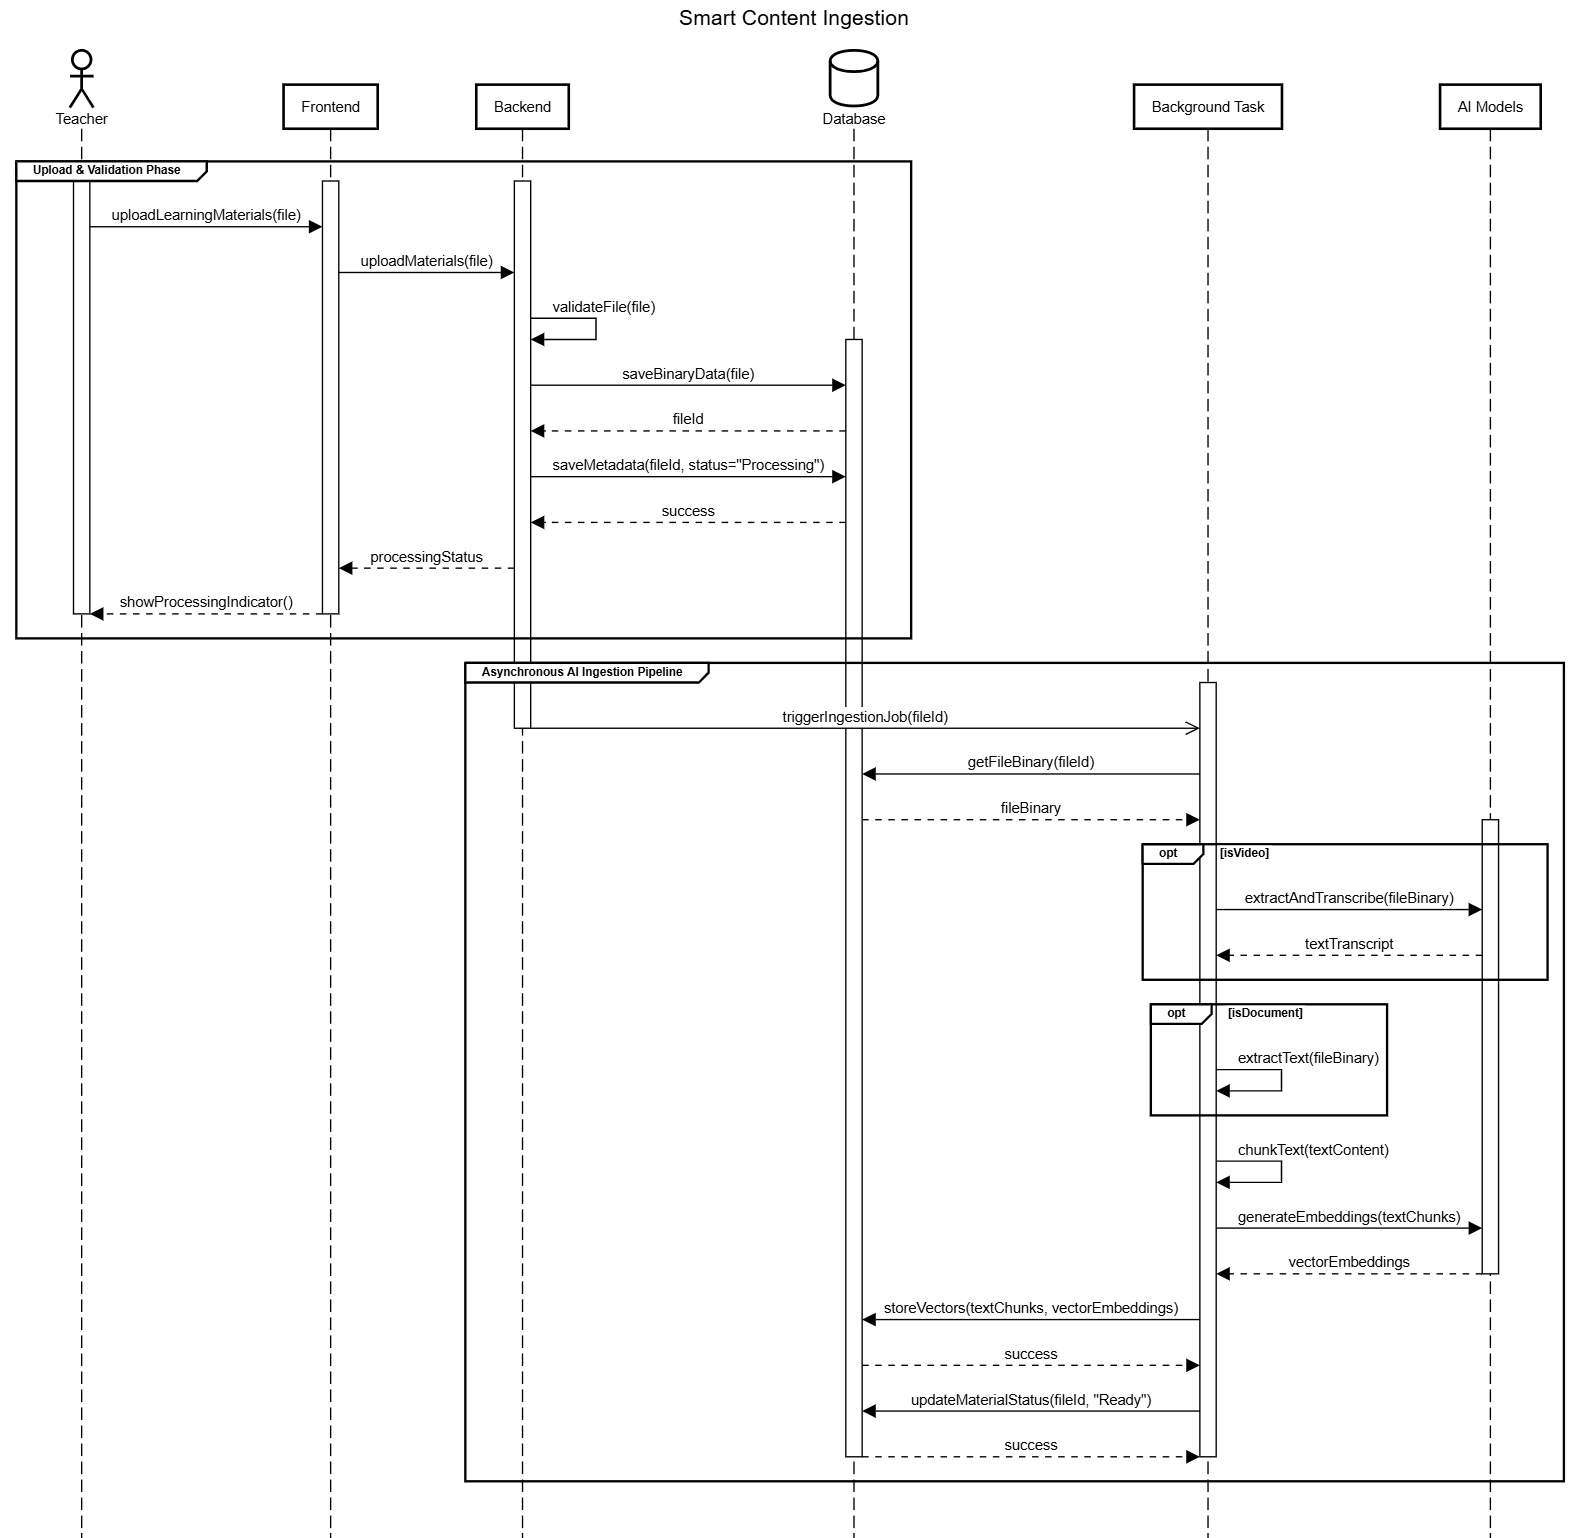
\includegraphics[width=1\textwidth]{graphics/seq-diagrams/seq_ingestion.png}
    \caption{Sequence Diagram: Smart Content Ingestion}
    \label{fig:seq_ingestion}
\end{figure}


\subsubsection{Human-in-the-Loop Quiz Generation}

This sequence diagram maps the assessment creation lifecycle, emphasizing the "Human-in-the-Loop" architectural pattern. While the AI Engine performs the computationally heavy task of generating questions via RAG based on the Course Knowledge Graph, the Teacher retains full control. The workflow includes a review and editing phase, allowing the instructor to adjust question content, difficulty levels, and passing thresholds before publishing the final quiz to the students.

\begin{figure}[H]
    \centering
    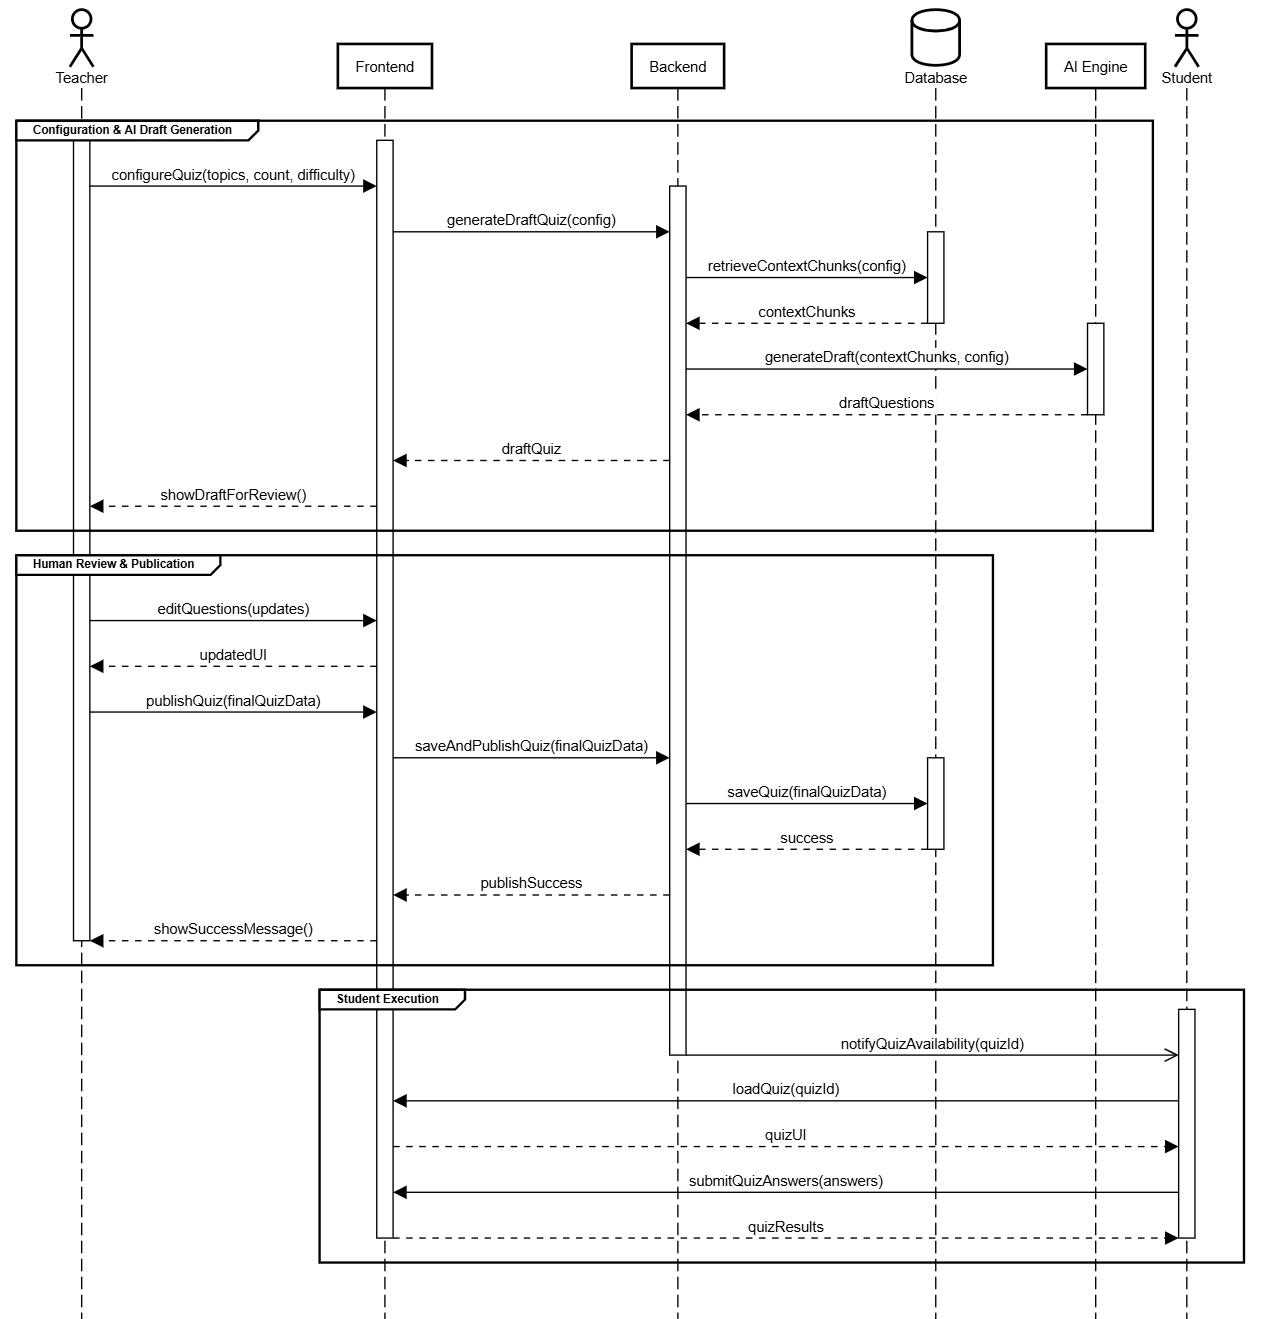
\includegraphics[width=0.95\textwidth]{graphics/seq-diagrams/seq_quiz_gen.png}
    \caption{Sequence Diagram: HITL Quiz Generation and Execution}
    \label{fig:seq_quiz_gen}
\end{figure}



\subsubsection{Native Mock Interview Session}
The current interview runtime is a stateful native LiveKit agent rather than the obsolete raster sequence previously included here. The diagram source for those figures is unavailable and their Qdrant/routed description no longer matches the implemented system; the following textual trace is therefore the authoritative specification.

\begin{enumerate}
    \item The learner starts or resumes a persisted session and completes onboarding. The API may mint a warm LiveKit token during setup, but dispatches the interviewer only after readiness.
    \item The browser joins the LiveKit room over WebRTC. FastAPI supplies ownership checks, room token, and dispatch metadata; it does not relay the audio media stream.
    \item The native worker loads durable runtime state and approved question candidates, then starts an \texttt{AgentSession} with STT, VAD, LLM, TTS, and persistent chat context.
    \item A spoken answer reaches the worker as a final STT transcript. A typed answer reaches \texttt{lk.chat}; its receipt is persisted before acknowledgement so retries reuse the idempotency key.
    \item The server folds the answer into provisional runtime state, persists it with optimistic versioning, and either advances to a server-selected question or records a bounded follow-up state. The LLM subsequently generates only the conversational wording.
    \item The worker publishes TTS audio, transcript, and ordered control snapshots. Deferred \texttt{arq} reconciliation improves provisional coverage; terminal evaluation independently judges the persisted transcript.
    \item A model completion request and the hard-stop timer converge on one finalization barrier that drains bounded in-flight work, submits once, queues evaluation, and closes the room after closing-audio playout.
\end{enumerate}

The full native implementation and authority boundary are described in Section~\ref{sec:impl_interviews}.